\batchmode
\documentclass[12pt,a4paper]{article}
\RequirePackage{ifthen}


\usepackage{amssymb}
\usepackage{graphicx}
\pagestyle{empty}
\textwidth = 15.5 cm
\textheight = 23.5 cm
\topmargin =-1.0 cm
\oddsidemargin = 0.5 cm
\listparindent=0pt
\itemsep=5pt



\usepackage{xcolor}

\usepackage[latin1]{inputenc}



\makeatletter

\makeatletter
\count@=\the\catcode`\_ \catcode`\_=8 
\newenvironment{tex2html_wrap}{}{}%
\catcode`\<=12\catcode`\_=\count@
\newcommand{\providedcommand}[1]{\expandafter\providecommand\csname #1\endcsname}%
\newcommand{\renewedcommand}[1]{\expandafter\providecommand\csname #1\endcsname{}%
  \expandafter\renewcommand\csname #1\endcsname}%
\newcommand{\newedenvironment}[1]{\newenvironment{#1}{}{}\renewenvironment{#1}}%
\let\newedcommand\renewedcommand
\let\renewedenvironment\newedenvironment
\makeatother
\let\mathon=$
\let\mathoff=$
\ifx\AtBeginDocument\undefined \newcommand{\AtBeginDocument}[1]{}\fi
\newbox\sizebox
\setlength{\hoffset}{0pt}\setlength{\voffset}{0pt}
\addtolength{\textheight}{\footskip}\setlength{\footskip}{0pt}
\addtolength{\textheight}{\topmargin}\setlength{\topmargin}{0pt}
\addtolength{\textheight}{\headheight}\setlength{\headheight}{0pt}
\addtolength{\textheight}{\headsep}\setlength{\headsep}{0pt}
\setlength{\textwidth}{349pt}
\newwrite\lthtmlwrite
\makeatletter
\let\realnormalsize=\normalsize
\global\topskip=2sp
\def\preveqno{}\let\real@float=\@float \let\realend@float=\end@float
\def\@float{\let\@savefreelist\@freelist\real@float}
\def\liih@math{\ifmmode$\else\bad@math\fi}
\def\end@float{\realend@float\global\let\@freelist\@savefreelist}
\let\real@dbflt=\@dbflt \let\end@dblfloat=\end@float
\let\@largefloatcheck=\relax
\let\if@boxedmulticols=\iftrue
\def\@dbflt{\let\@savefreelist\@freelist\real@dbflt}
\def\adjustnormalsize{\def\normalsize{\mathsurround=0pt \realnormalsize
 \parindent=0pt\abovedisplayskip=0pt\belowdisplayskip=0pt}%
 \def\phantompar{\csname par\endcsname}\normalsize}%
\def\lthtmltypeout#1{{\let\protect\string \immediate\write\lthtmlwrite{#1}}}%
\newcommand\lthtmlhboxmathA{\adjustnormalsize\setbox\sizebox=\hbox\bgroup\kern.05em }%
\newcommand\lthtmlhboxmathB{\adjustnormalsize\setbox\sizebox=\hbox to\hsize\bgroup\hfill }%
\newcommand\lthtmlvboxmathA{\adjustnormalsize\setbox\sizebox=\vbox\bgroup %
 \let\ifinner=\iffalse \let\)\liih@math }%
\newcommand\lthtmlboxmathZ{\@next\next\@currlist{}{\def\next{\voidb@x}}%
 \expandafter\box\next\egroup}%
\newcommand\lthtmlmathtype[1]{\gdef\lthtmlmathenv{#1}}%
\newcommand\lthtmllogmath{\dimen0\ht\sizebox \advance\dimen0\dp\sizebox
  \ifdim\dimen0>.95\vsize
   \lthtmltypeout{%
*** image for \lthtmlmathenv\space is too tall at \the\dimen0, reducing to .95 vsize ***}%
   \ht\sizebox.95\vsize \dp\sizebox\z@ \fi
  \lthtmltypeout{l2hSize %
:\lthtmlmathenv:\the\ht\sizebox::\the\dp\sizebox::\the\wd\sizebox.\preveqno}}%
\newcommand\lthtmlfigureA[1]{\let\@savefreelist\@freelist
       \lthtmlmathtype{#1}\lthtmlvboxmathA}%
\newcommand\lthtmlpictureA{\bgroup\catcode`\_=8 \lthtmlpictureB}%
\newcommand\lthtmlpictureB[1]{\lthtmlmathtype{#1}\egroup
       \let\@savefreelist\@freelist \lthtmlhboxmathB}%
\newcommand\lthtmlpictureZ[1]{\hfill\lthtmlfigureZ}%
\newcommand\lthtmlfigureZ{\lthtmlboxmathZ\lthtmllogmath\copy\sizebox
       \global\let\@freelist\@savefreelist}%
\newcommand\lthtmldisplayA{\bgroup\catcode`\_=8 \lthtmldisplayAi}%
\newcommand\lthtmldisplayAi[1]{\lthtmlmathtype{#1}\egroup\lthtmlvboxmathA}%
\newcommand\lthtmldisplayB[1]{\edef\preveqno{(\theequation)}%
  \lthtmldisplayA{#1}\let\@eqnnum\relax}%
\newcommand\lthtmldisplayZ{\lthtmlboxmathZ\lthtmllogmath\lthtmlsetmath}%
\newcommand\lthtmlinlinemathA{\bgroup\catcode`\_=8 \lthtmlinlinemathB}
\newcommand\lthtmlinlinemathB[1]{\lthtmlmathtype{#1}\egroup\lthtmlhboxmathA
  \vrule height1.5ex width0pt }%
\newcommand\lthtmlinlineA{\bgroup\catcode`\_=8 \lthtmlinlineB}%
\newcommand\lthtmlinlineB[1]{\lthtmlmathtype{#1}\egroup\lthtmlhboxmathA}%
\newcommand\lthtmlinlineZ{\egroup\expandafter\ifdim\dp\sizebox>0pt %
  \expandafter\centerinlinemath\fi\lthtmllogmath\lthtmlsetinline}
\newcommand\lthtmlinlinemathZ{\egroup\expandafter\ifdim\dp\sizebox>0pt %
  \expandafter\centerinlinemath\fi\lthtmllogmath\lthtmlsetmath}
\newcommand\lthtmlindisplaymathZ{\egroup %
  \centerinlinemath\lthtmllogmath\lthtmlsetmath}
\def\lthtmlsetinline{\hbox{\vrule width.1em \vtop{\vbox{%
  \kern.1em\copy\sizebox}\ifdim\dp\sizebox>0pt\kern.1em\else\kern.3pt\fi
  \ifdim\hsize>\wd\sizebox \hrule depth1pt\fi}}}
\def\lthtmlsetmath{\hbox{\vrule width.1em\kern-.05em\vtop{\vbox{%
  \kern.1em\kern0.8 pt\hbox{\hglue.17em\copy\sizebox\hglue0.8 pt}}\kern.3pt%
  \ifdim\dp\sizebox>0pt\kern.1em\fi \kern0.8 pt%
  \ifdim\hsize>\wd\sizebox \hrule depth1pt\fi}}}
\def\centerinlinemath{%
  \dimen1=\ifdim\ht\sizebox<\dp\sizebox \dp\sizebox\else\ht\sizebox\fi
  \advance\dimen1by.5pt \vrule width0pt height\dimen1 depth\dimen1 
 \dp\sizebox=\dimen1\ht\sizebox=\dimen1\relax}

\def\lthtmlcheckvsize{\ifdim\ht\sizebox<\vsize 
  \ifdim\wd\sizebox<\hsize\expandafter\hfill\fi \expandafter\vfill
  \else\expandafter\vss\fi}%
\providecommand{\selectlanguage}[1]{}%
\makeatletter \tracingstats = 1 
\providecommand{\Omicron}{\textrm{O}}
\providecommand{\Mu}{\textrm{M}}
\providecommand{\Rho}{\textrm{R}}
\providecommand{\Nu}{\textrm{N}}
\providecommand{\Zeta}{\textrm{Z}}
\providecommand{\Chi}{\textrm{X}}
\providecommand{\Eta}{\textrm{H}}
\providecommand{\Beta}{\textrm{B}}
\providecommand{\Iota}{\textrm{J}}
\providecommand{\omicron}{\textrm{o}}
\providecommand{\Kappa}{\textrm{K}}
\providecommand{\Alpha}{\textrm{A}}
\providecommand{\Tau}{\textrm{T}}
\providecommand{\Epsilon}{\textrm{E}}


\begin{document}
\pagestyle{empty}\thispagestyle{empty}\lthtmltypeout{}%
\lthtmltypeout{latex2htmlLength hsize=\the\hsize}\lthtmltypeout{}%
\lthtmltypeout{latex2htmlLength vsize=\the\vsize}\lthtmltypeout{}%
\lthtmltypeout{latex2htmlLength hoffset=\the\hoffset}\lthtmltypeout{}%
\lthtmltypeout{latex2htmlLength voffset=\the\voffset}\lthtmltypeout{}%
\lthtmltypeout{latex2htmlLength topmargin=\the\topmargin}\lthtmltypeout{}%
\lthtmltypeout{latex2htmlLength topskip=\the\topskip}\lthtmltypeout{}%
\lthtmltypeout{latex2htmlLength headheight=\the\headheight}\lthtmltypeout{}%
\lthtmltypeout{latex2htmlLength headsep=\the\headsep}\lthtmltypeout{}%
\lthtmltypeout{latex2htmlLength parskip=\the\parskip}\lthtmltypeout{}%
\lthtmltypeout{latex2htmlLength oddsidemargin=\the\oddsidemargin}\lthtmltypeout{}%
\makeatletter
\if@twoside\lthtmltypeout{latex2htmlLength evensidemargin=\the\evensidemargin}%
\else\lthtmltypeout{latex2htmlLength evensidemargin=\the\oddsidemargin}\fi%
\lthtmltypeout{}%
\makeatother
\setcounter{page}{1}
\onecolumn

% !!! IMAGES START HERE !!!

{\newpage\clearpage
\lthtmlinlinemathA{tex2html_wrap_inline1495}%
$ \thicksim$%
\lthtmlinlinemathZ
\lthtmlcheckvsize\clearpage}

\stepcounter{section}
\stepcounter{subsection}
\stepcounter{subsection}
\stepcounter{subsection}
\stepcounter{section}
\stepcounter{subsection}
\stepcounter{subsubsection}
{\newpage\clearpage
\lthtmlinlinemathA{tex2html_wrap_inline1518}%
$ \rho$%
\lthtmlinlinemathZ
\lthtmlcheckvsize\clearpage}

{\newpage\clearpage
\lthtmlinlinemathA{tex2html_wrap_inline1519}%
$ \rightarrow$%
\lthtmlinlinemathZ
\lthtmlcheckvsize\clearpage}

{\newpage\clearpage
\lthtmlinlinemathA{tex2html_wrap_inline1523}%
$ \alpha$%
\lthtmlinlinemathZ
\lthtmlcheckvsize\clearpage}

{\newpage\clearpage
\lthtmlinlinemathA{tex2html_wrap_inline1526}%
$ \infty$%
\lthtmlinlinemathZ
\lthtmlcheckvsize\clearpage}

\stepcounter{subsubsection}
\stepcounter{subsubsection}
\stepcounter{subsubsection}
{\newpage\clearpage
\lthtmlinlinemathA{tex2html_wrap_inline1606}%
$ \ge$%
\lthtmlinlinemathZ
\lthtmlcheckvsize\clearpage}

{\newpage\clearpage
\lthtmlinlinemathA{tex2html_wrap_inline1610}%
$ \rho_{c}^{}$%
\lthtmlinlinemathZ
\lthtmlcheckvsize\clearpage}

{\newpage\clearpage
\lthtmlinlinemathA{tex2html_wrap_inline1612}%
$ \rho_{v}^{}$%
\lthtmlinlinemathZ
\lthtmlcheckvsize\clearpage}

{\newpage\clearpage
\lthtmlinlinemathA{tex2html_wrap_inline1615}%
$ \sim$%
\lthtmlinlinemathZ
\lthtmlcheckvsize\clearpage}

\stepcounter{subsection}
\stepcounter{subsubsection}
\stepcounter{subsubsection}
\stepcounter{subsubsection}
\stepcounter{subsection}
\stepcounter{subsection}
\stepcounter{section}
\stepcounter{subsection}
\stepcounter{subsubsection}
{\newpage\clearpage
\lthtmlpictureA{tex2html_wrap1745}%
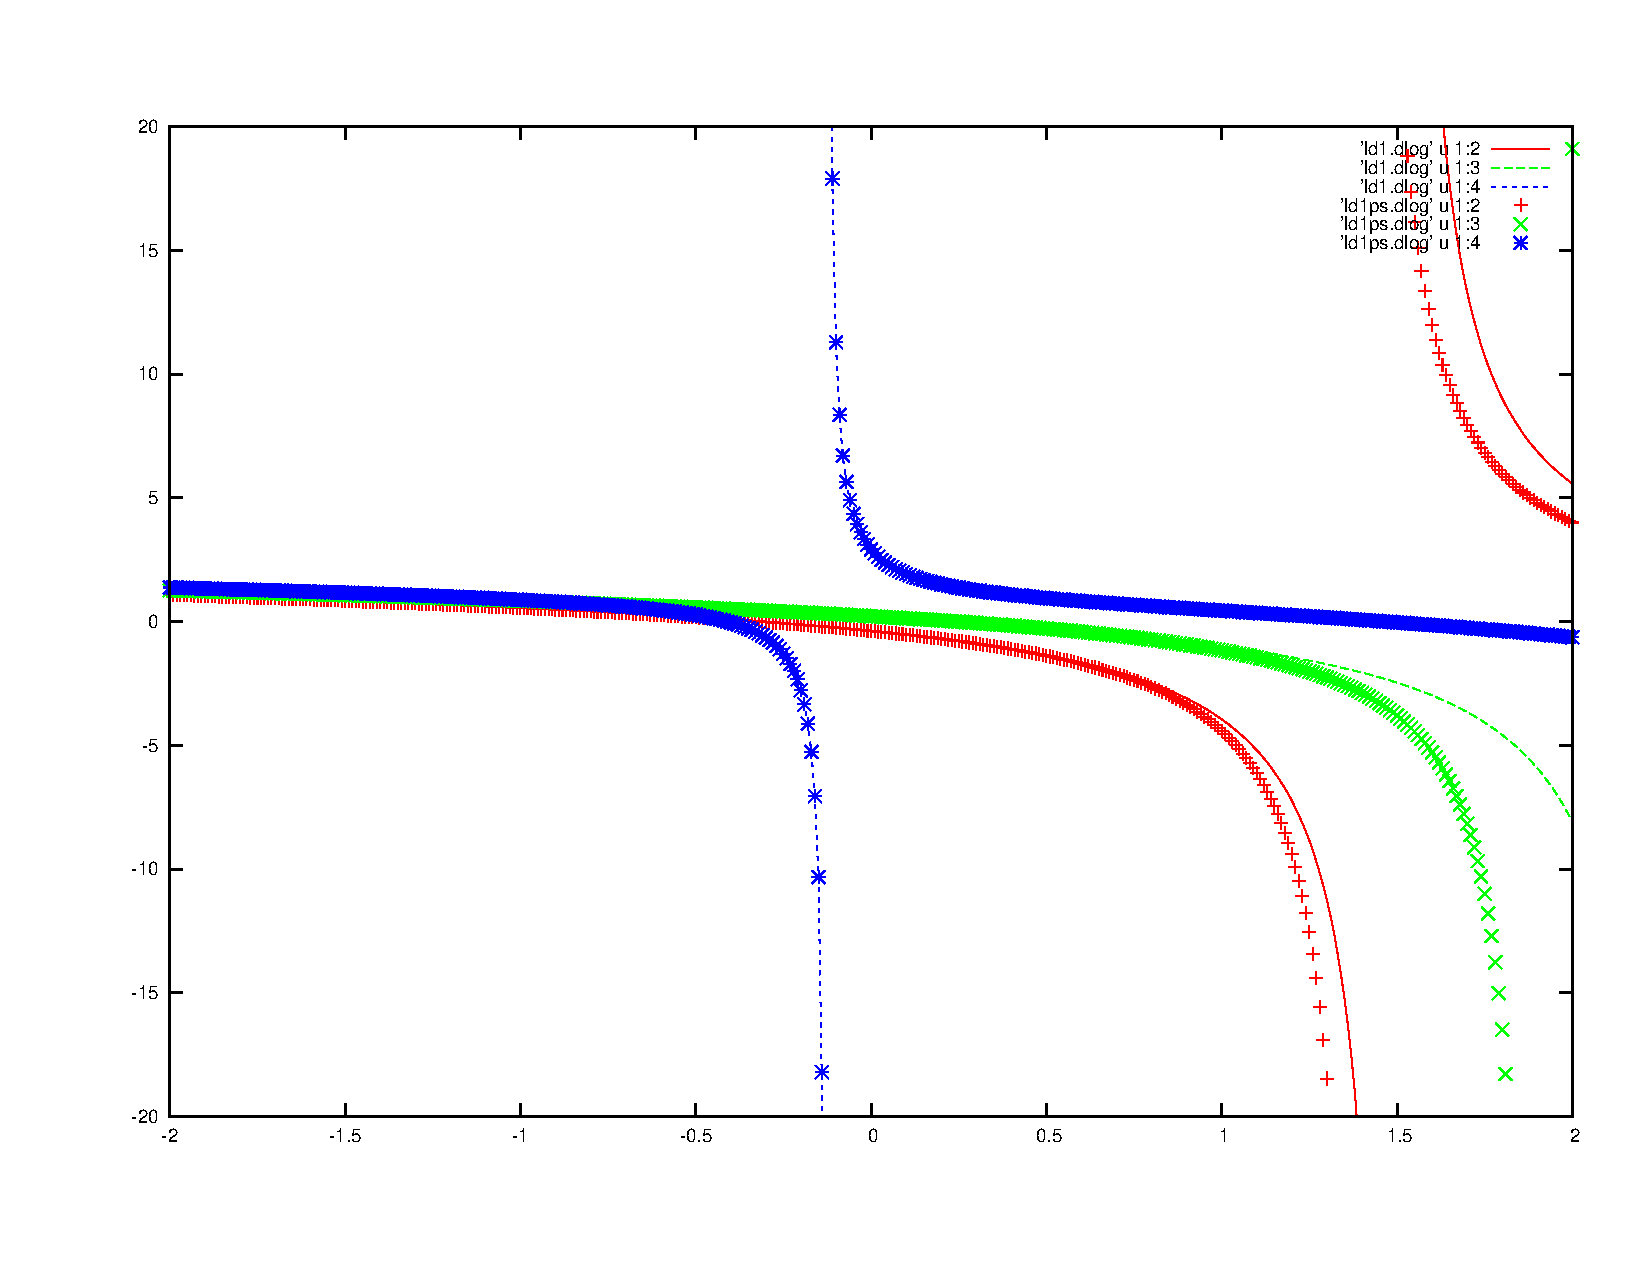
\includegraphics[width=7.5cm]{pseudo-gen-fig1.pdf}%
\lthtmlpictureZ
\lthtmlcheckvsize\clearpage}

{\newpage\clearpage
\lthtmlpictureA{tex2html_wrap1746}%
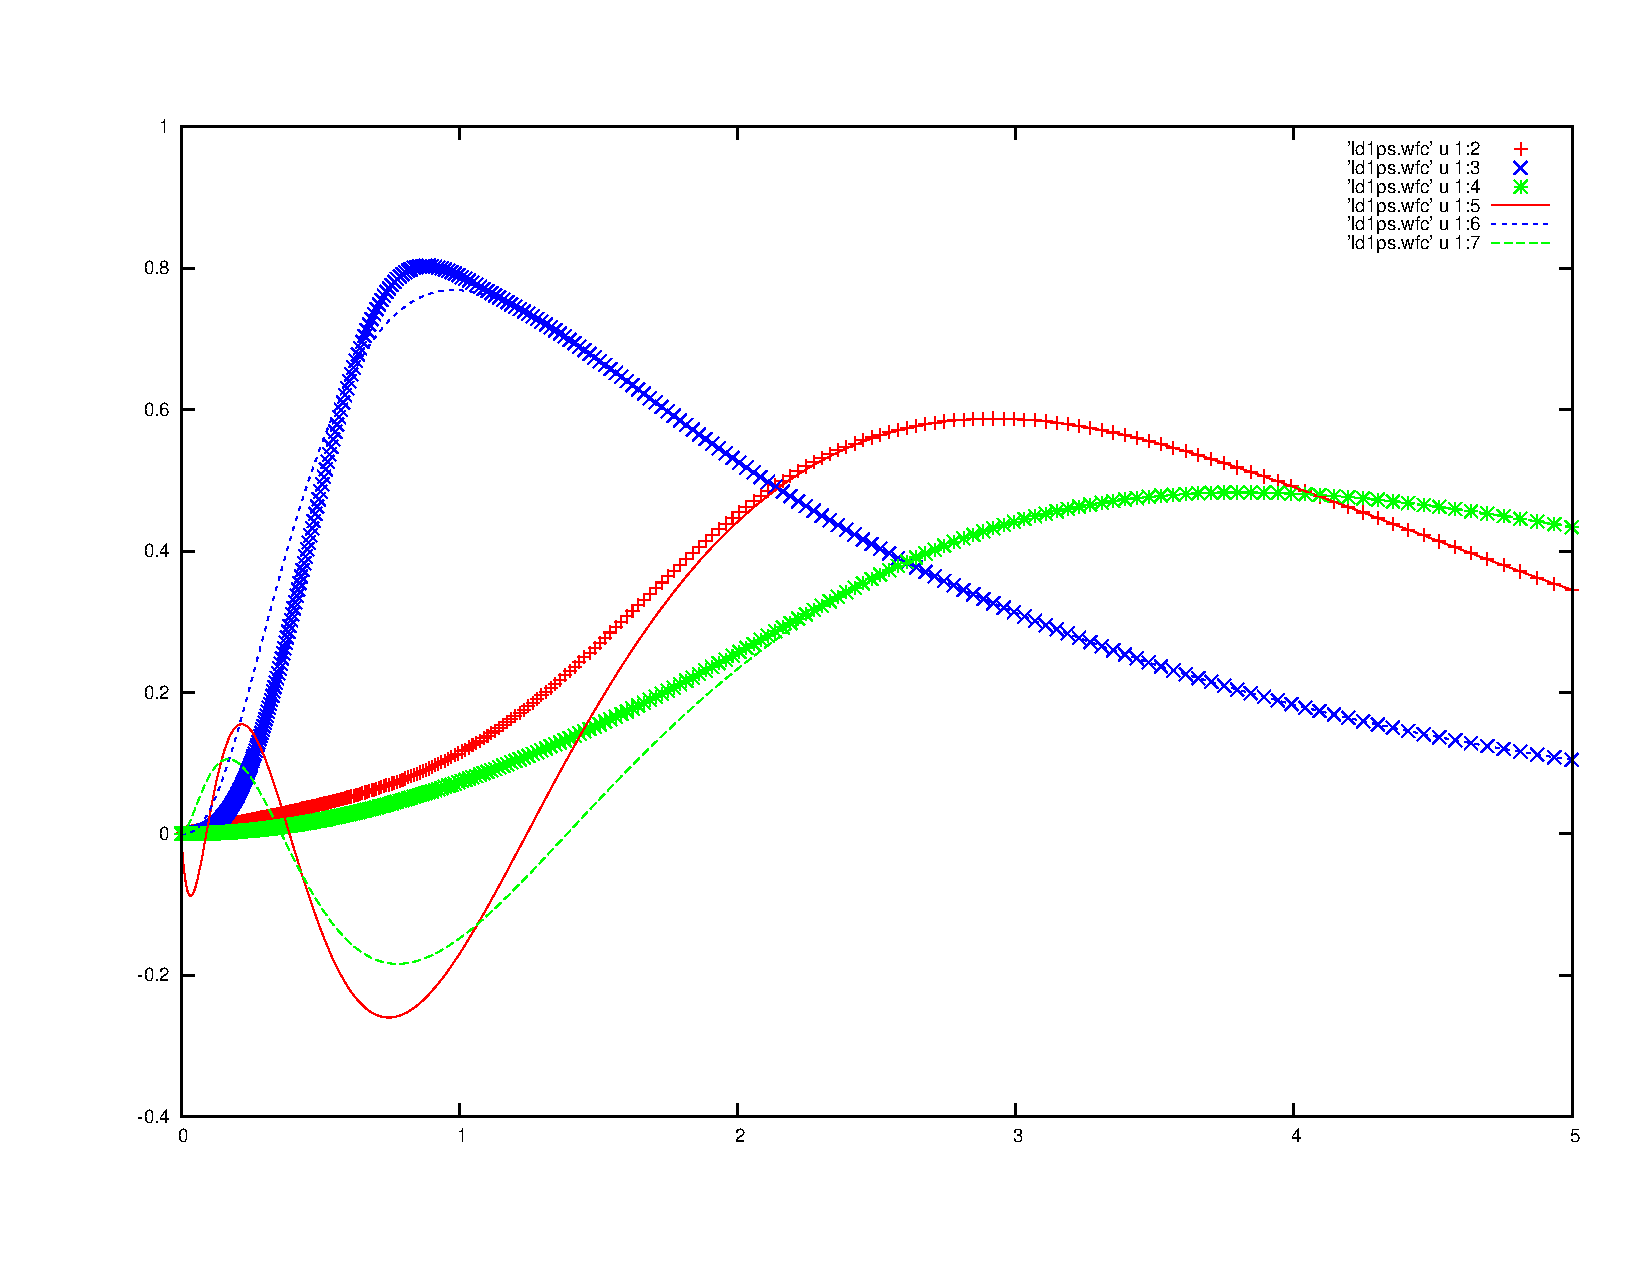
\includegraphics[width=7.5cm]{pseudo-gen-fig2.pdf}%
\lthtmlpictureZ
\lthtmlcheckvsize\clearpage}

\stepcounter{subsubsection}
{\newpage\clearpage
\lthtmlinlinemathA{tex2html_wrap_inline1756}%
$ \delta$%
\lthtmlinlinemathZ
\lthtmlcheckvsize\clearpage}

{\newpage\clearpage
\lthtmlpictureA{tex2html_wrap1774}%
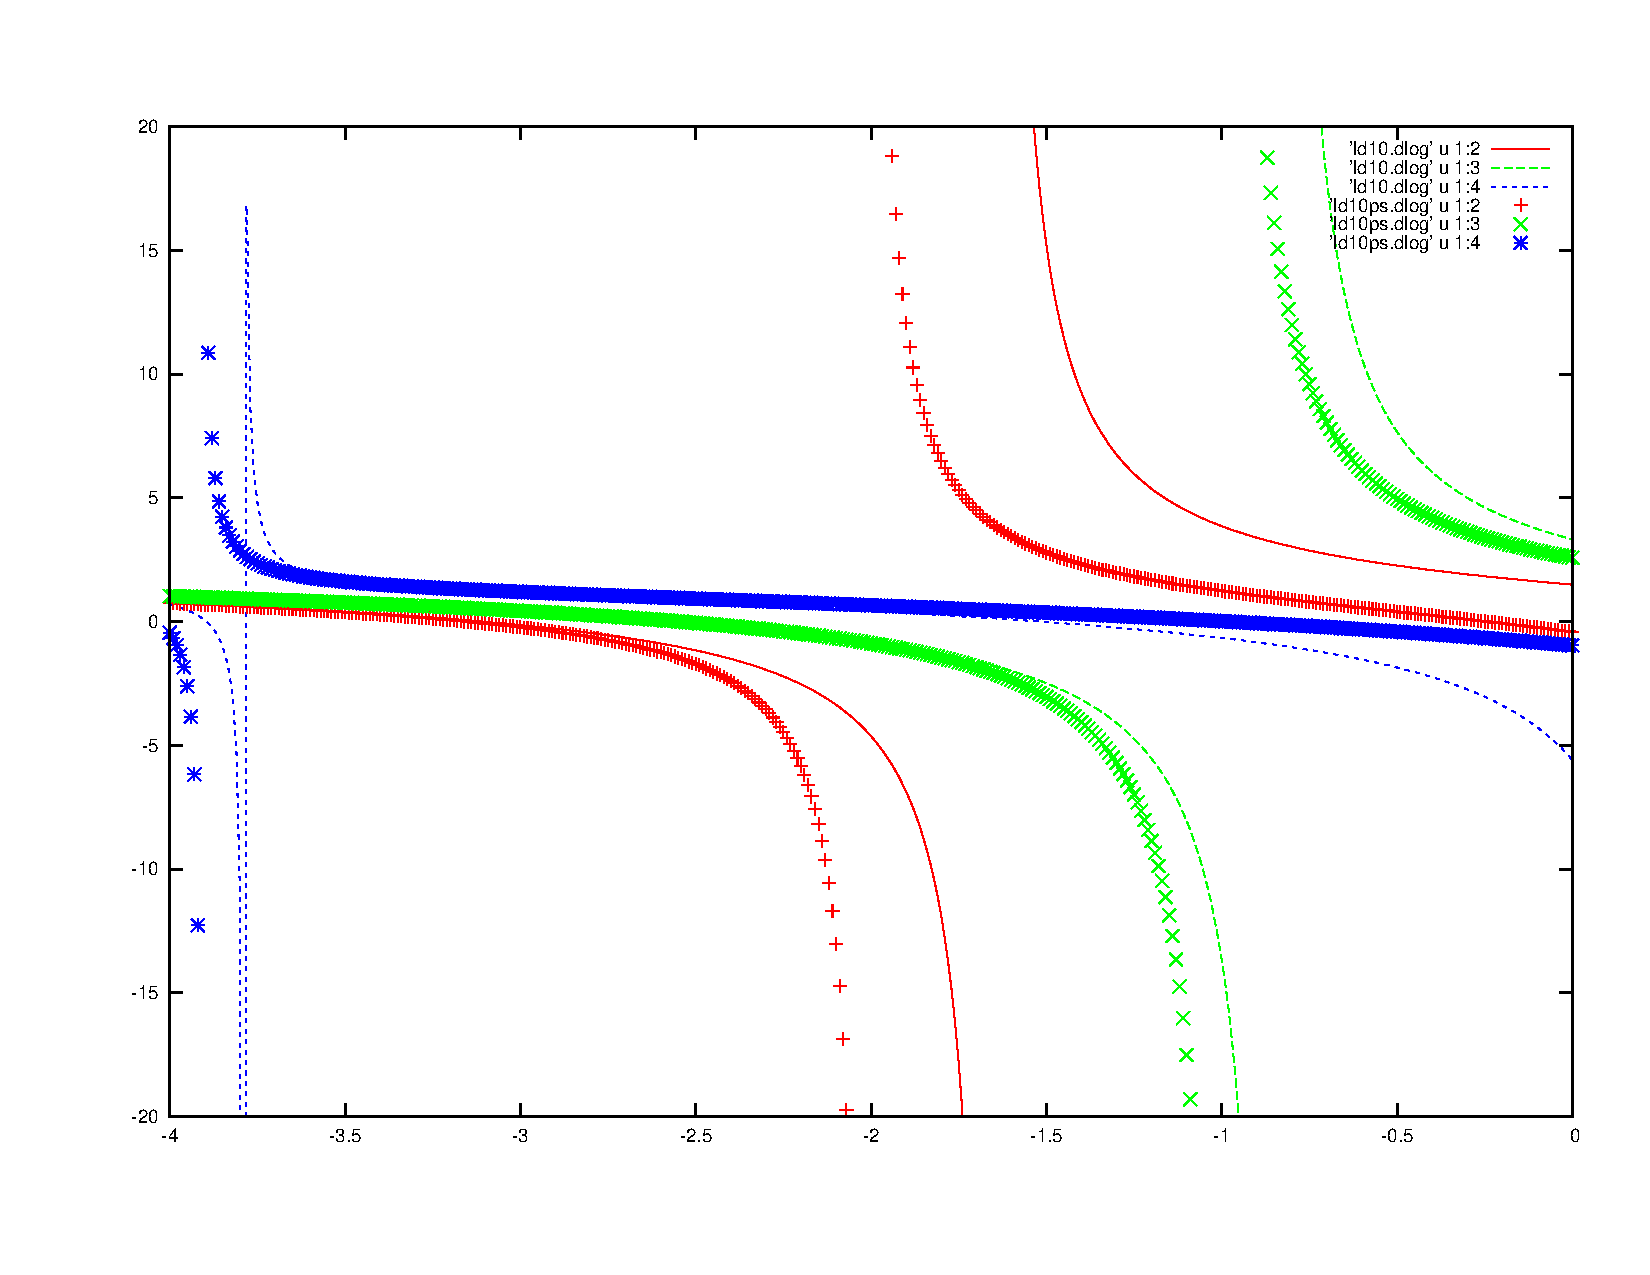
\includegraphics[width=7.5cm]{pseudo-gen-fig3.pdf}%
\lthtmlpictureZ
\lthtmlcheckvsize\clearpage}

{\newpage\clearpage
\lthtmlpictureA{tex2html_wrap1775}%
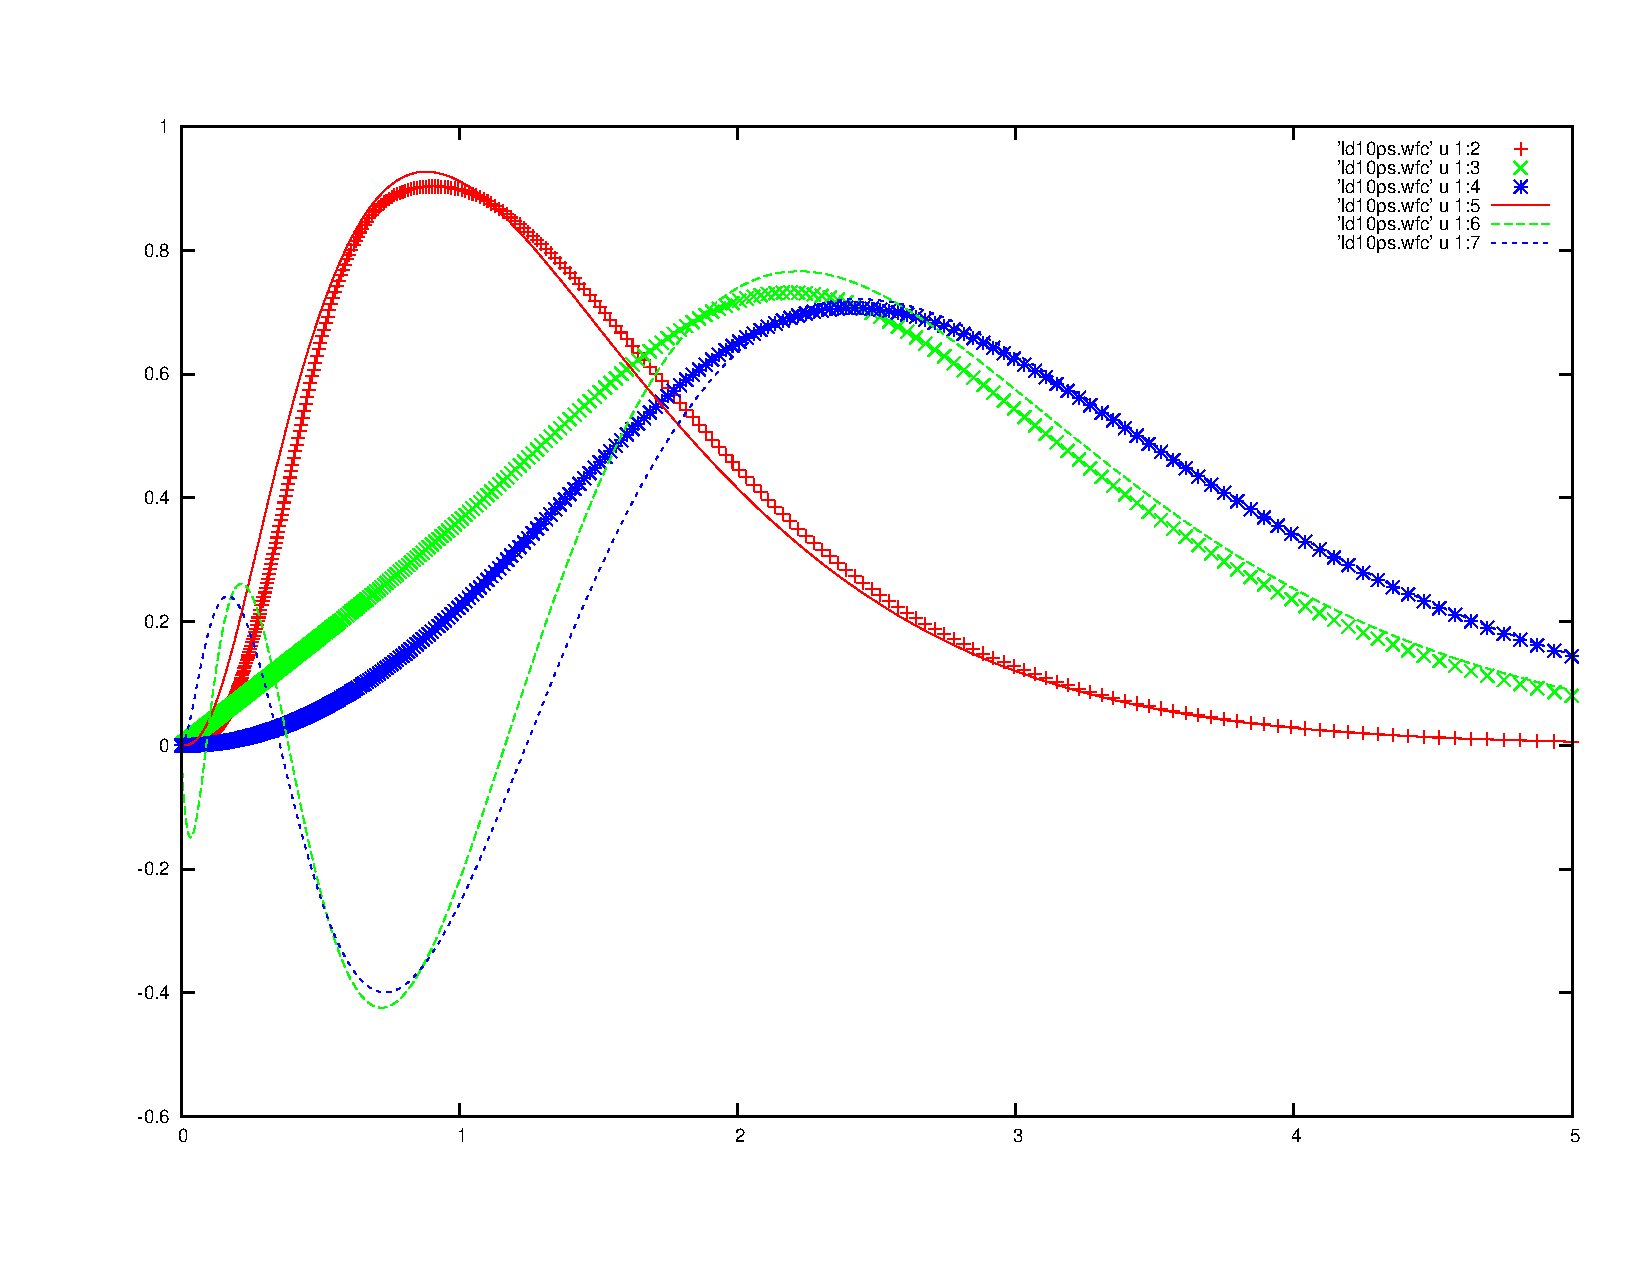
\includegraphics[width=7.5cm]{pseudo-gen-fig4.pdf}%
\lthtmlpictureZ
\lthtmlcheckvsize\clearpage}

\stepcounter{subsection}
\stepcounter{subsection}
\appendix
\stepcounter{section}
\stepcounter{subsection}
{\newpage\clearpage
\lthtmlinlinemathA{tex2html_wrap_indisplay1807}%
$\displaystyle \left(\vphantom{-{\hbar^2\over 2m}\nabla^2 + V(r)-\epsilon}\right.$%
\lthtmlindisplaymathZ
\lthtmlcheckvsize\clearpage}

{\newpage\clearpage
\lthtmlinlinemathA{tex2html_wrap_indisplay1808}%
$\displaystyle {\hbar^2\over 2m}$%
\lthtmlindisplaymathZ
\lthtmlcheckvsize\clearpage}

{\newpage\clearpage
\lthtmlinlinemathA{tex2html_wrap_indisplay1809}%
$\displaystyle \nabla^{2}_{}$%
\lthtmlindisplaymathZ
\lthtmlcheckvsize\clearpage}

{\newpage\clearpage
\lthtmlinlinemathA{tex2html_wrap_indisplay1810}%
$\displaystyle \epsilon$%
\lthtmlindisplaymathZ
\lthtmlcheckvsize\clearpage}

{\newpage\clearpage
\lthtmlinlinemathA{tex2html_wrap_indisplay1811}%
$\displaystyle \left.\vphantom{-{\hbar^2\over 2m}\nabla^2 + V(r)-\epsilon}\right)$%
\lthtmlindisplaymathZ
\lthtmlcheckvsize\clearpage}

{\newpage\clearpage
\lthtmlinlinemathA{tex2html_wrap_indisplay1812}%
$\displaystyle \psi$%
\lthtmlindisplaymathZ
\lthtmlcheckvsize\clearpage}

{\newpage\clearpage
\lthtmlinlinemathA{tex2html_wrap_indisplay1813}%
$\displaystyle \bf r$%
\lthtmlindisplaymathZ
\lthtmlcheckvsize\clearpage}

{\newpage\clearpage
\lthtmlinlinemathA{tex2html_wrap_indisplay1817}%
$\displaystyle \left(\vphantom{{R_{nl}(r)\over r}}\right.$%
\lthtmlindisplaymathZ
\lthtmlcheckvsize\clearpage}

{\newpage\clearpage
\lthtmlinlinemathA{tex2html_wrap_indisplay1818}%
$\displaystyle {R_{nl}(r)\over r}$%
\lthtmlindisplaymathZ
\lthtmlcheckvsize\clearpage}

{\newpage\clearpage
\lthtmlinlinemathA{tex2html_wrap_indisplay1819}%
$\displaystyle \left.\vphantom{{R_{nl}(r)\over r}}\right)$%
\lthtmlindisplaymathZ
\lthtmlcheckvsize\clearpage}

{\newpage\clearpage
\lthtmlinlinemathA{tex2html_wrap_indisplay1820}%
$\displaystyle \hat{{\bf r}}$%
\lthtmlindisplaymathZ
\lthtmlcheckvsize\clearpage}

{\newpage\clearpage
\lthtmlinlinemathA{tex2html_wrap_indisplay1826}%
$\displaystyle \left(\vphantom{-{\hbar^2\over 2m} {1\over r} {d^2 R_{nl}(r)\over dr^2}
+(V(r)-\epsilon) {1\over r} R_{nl}(r)
}\right.$%
\lthtmlindisplaymathZ
\lthtmlcheckvsize\clearpage}

{\newpage\clearpage
\lthtmlinlinemathA{tex2html_wrap_indisplay1828}%
$\displaystyle {1\over r}$%
\lthtmlindisplaymathZ
\lthtmlcheckvsize\clearpage}

{\newpage\clearpage
\lthtmlinlinemathA{tex2html_wrap_indisplay1829}%
$\displaystyle {d^2 R_{nl}(r)\over dr^2}$%
\lthtmlindisplaymathZ
\lthtmlcheckvsize\clearpage}

{\newpage\clearpage
\lthtmlinlinemathA{tex2html_wrap_indisplay1832}%
$\displaystyle \left.\vphantom{-{\hbar^2\over 2m} {1\over r} {d^2 R_{nl}(r)\over dr^2}
+(V(r)-\epsilon) {1\over r} R_{nl}(r)
}\right)$%
\lthtmlindisplaymathZ
\lthtmlcheckvsize\clearpage}

{\newpage\clearpage
\lthtmlinlinemathA{tex2html_wrap_indisplay1836}%
$\displaystyle \left(\vphantom{{1\over\mbox{sin}\theta}{\partial\over\partial\theta}
\left(\mbox{sin}\theta{\partial Y_{lm}(\hat{\bf r})
\over\partial\theta}\right)
+ {1\over\mbox{sin}^2\theta}
{\partial^2Y_{lm}(\hat{\bf r})\over\partial\phi^2}
}\right.$%
\lthtmlindisplaymathZ
\lthtmlcheckvsize\clearpage}

{\newpage\clearpage
\lthtmlinlinemathA{tex2html_wrap_indisplay1837}%
$\displaystyle {1\over\mbox{sin}\theta}$%
\lthtmlindisplaymathZ
\lthtmlcheckvsize\clearpage}

{\newpage\clearpage
\lthtmlinlinemathA{tex2html_wrap_indisplay1838}%
$\displaystyle {\partial\over\partial\theta}$%
\lthtmlindisplaymathZ
\lthtmlcheckvsize\clearpage}

{\newpage\clearpage
\lthtmlinlinemathA{tex2html_wrap_indisplay1839}%
$\displaystyle \left(\vphantom{\mbox{sin}\theta{\partial Y_{lm}(\hat{\bf r})
\over\partial\theta}}\right.$%
\lthtmlindisplaymathZ
\lthtmlcheckvsize\clearpage}

{\newpage\clearpage
\lthtmlinlinemathA{tex2html_wrap_indisplay1840}%
$\displaystyle \theta$%
\lthtmlindisplaymathZ
\lthtmlcheckvsize\clearpage}

{\newpage\clearpage
\lthtmlinlinemathA{tex2html_wrap_indisplay1841}%
$\displaystyle {\partial Y_{lm}(\hat{\bf r})
\over\partial\theta}$%
\lthtmlindisplaymathZ
\lthtmlcheckvsize\clearpage}

{\newpage\clearpage
\lthtmlinlinemathA{tex2html_wrap_indisplay1842}%
$\displaystyle \left.\vphantom{\mbox{sin}\theta{\partial Y_{lm}(\hat{\bf r})
\over\partial\theta}}\right)$%
\lthtmlindisplaymathZ
\lthtmlcheckvsize\clearpage}

{\newpage\clearpage
\lthtmlinlinemathA{tex2html_wrap_indisplay1843}%
$\displaystyle {1\over\mbox{sin}^2\theta}$%
\lthtmlindisplaymathZ
\lthtmlcheckvsize\clearpage}

{\newpage\clearpage
\lthtmlinlinemathA{tex2html_wrap_indisplay1844}%
$\displaystyle {\partial^2Y_{lm}(\hat{\bf r})\over\partial\phi^2}$%
\lthtmlindisplaymathZ
\lthtmlcheckvsize\clearpage}

{\newpage\clearpage
\lthtmlinlinemathA{tex2html_wrap_indisplay1845}%
$\displaystyle \left.\vphantom{{1\over\mbox{sin}\theta}{\partial\over\partial\theta}
\left(\mbox{sin}\theta{\partial Y_{lm}(\hat{\bf r})
\over\partial\theta}\right)
+ {1\over\mbox{sin}^2\theta}
{\partial^2Y_{lm}(\hat{\bf r})\over\partial\phi^2}
}\right)$%
\lthtmlindisplaymathZ
\lthtmlcheckvsize\clearpage}

{\newpage\clearpage
\lthtmlinlinemathA{tex2html_wrap_indisplay1846}%
$\displaystyle {1\over r^3}$%
\lthtmlindisplaymathZ
\lthtmlcheckvsize\clearpage}

{\newpage\clearpage
\lthtmlinlinemathA{tex2html_wrap_inline1848}%
$ \hat{{\bf r}}$%
\lthtmlinlinemathZ
\lthtmlcheckvsize\clearpage}

{\newpage\clearpage
\lthtmlinlinemathA{tex2html_wrap_indisplay1865}%
$\displaystyle \left(\vphantom{ {\hbar^2\over 2m} {l(l+1)\over r^2} + V(r)-\epsilon
}\right.$%
\lthtmlindisplaymathZ
\lthtmlcheckvsize\clearpage}

{\newpage\clearpage
\lthtmlinlinemathA{tex2html_wrap_indisplay1867}%
$\displaystyle {l(l+1)\over r^2}$%
\lthtmlindisplaymathZ
\lthtmlcheckvsize\clearpage}

{\newpage\clearpage
\lthtmlinlinemathA{tex2html_wrap_indisplay1869}%
$\displaystyle \left.\vphantom{ {\hbar^2\over 2m} {l(l+1)\over r^2} + V(r)-\epsilon
}\right)$%
\lthtmlindisplaymathZ
\lthtmlcheckvsize\clearpage}

{\newpage\clearpage
\lthtmlinlinemathA{tex2html_wrap_indisplay1871}%
$\displaystyle \sum_{{nlm}}^{}$%
\lthtmlindisplaymathZ
\lthtmlcheckvsize\clearpage}

{\newpage\clearpage
\lthtmlinlinemathA{tex2html_wrap_indisplay1872}%
$\displaystyle \Theta_{{nl}}^{}$%
\lthtmlindisplaymathZ
\lthtmlcheckvsize\clearpage}

{\newpage\clearpage
\lthtmlinlinemathA{tex2html_wrap_indisplay1873}%
$\displaystyle \left|\vphantom{{R_{nl}(r)\over r}Y_{lm}(\hat r)}\right.$%
\lthtmlindisplaymathZ
\lthtmlcheckvsize\clearpage}

{\newpage\clearpage
\lthtmlinlinemathA{tex2html_wrap_indisplay1875}%
$\displaystyle \hat{r}$%
\lthtmlindisplaymathZ
\lthtmlcheckvsize\clearpage}

{\newpage\clearpage
\lthtmlinlinemathA{tex2html_wrap_indisplay1876}%
$\displaystyle \left.\vphantom{{R_{nl}(r)\over r}Y_{lm}(\hat r)}\right|^{2}_{}$%
\lthtmlindisplaymathZ
\lthtmlcheckvsize\clearpage}

{\newpage\clearpage
\lthtmlinlinemathA{tex2html_wrap_indisplay1877}%
$\displaystyle \sum_{{nl}}^{}$%
\lthtmlindisplaymathZ
\lthtmlcheckvsize\clearpage}

{\newpage\clearpage
\lthtmlinlinemathA{tex2html_wrap_indisplay1879}%
$\displaystyle {R^2_{nl}(r)\over 4\pi r^2}$%
\lthtmlindisplaymathZ
\lthtmlcheckvsize\clearpage}

{\newpage\clearpage
\lthtmlinlinemathA{tex2html_wrap_inline1881}%
$ \Theta_{{nl}}^{}$%
\lthtmlinlinemathZ
\lthtmlcheckvsize\clearpage}

{\newpage\clearpage
\lthtmlinlinemathA{tex2html_wrap_inline1884}%
$ \le$%
\lthtmlinlinemathZ
\lthtmlcheckvsize\clearpage}

\stepcounter{subsubsection}
{\newpage\clearpage
\lthtmlinlinemathA{tex2html_wrap_inline1888}%
$ \theta$%
\lthtmlinlinemathZ
\lthtmlcheckvsize\clearpage}

{\newpage\clearpage
\lthtmlinlinemathA{tex2html_wrap_inline1889}%
$ \phi$%
\lthtmlinlinemathZ
\lthtmlcheckvsize\clearpage}

{\newpage\clearpage
\lthtmlinlinemathA{tex2html_wrap_indisplay1891}%
$\displaystyle \nabla$%
\lthtmlindisplaymathZ
\lthtmlcheckvsize\clearpage}

{\newpage\clearpage
\lthtmlinlinemathA{tex2html_wrap_indisplay1893}%
$\displaystyle \left(\vphantom{{\partial\psi\over\partial r},
                   {1\over r}{\partial\psi\over\partial\theta},
                   {1\over r \mbox{sin}\theta}
                              {\partial\psi\over\partial\phi}
             }\right.$%
\lthtmlindisplaymathZ
\lthtmlcheckvsize\clearpage}

{\newpage\clearpage
\lthtmlinlinemathA{tex2html_wrap_indisplay1894}%
$\displaystyle {\partial\psi\over\partial r}$%
\lthtmlindisplaymathZ
\lthtmlcheckvsize\clearpage}

{\newpage\clearpage
\lthtmlinlinemathA{tex2html_wrap_indisplay1896}%
$\displaystyle {\partial\psi\over\partial\theta}$%
\lthtmlindisplaymathZ
\lthtmlcheckvsize\clearpage}

{\newpage\clearpage
\lthtmlinlinemathA{tex2html_wrap_indisplay1897}%
$\displaystyle {1\over r \mbox{sin}\theta}$%
\lthtmlindisplaymathZ
\lthtmlcheckvsize\clearpage}

{\newpage\clearpage
\lthtmlinlinemathA{tex2html_wrap_indisplay1898}%
$\displaystyle {\partial\psi\over\partial\phi}$%
\lthtmlindisplaymathZ
\lthtmlcheckvsize\clearpage}

{\newpage\clearpage
\lthtmlinlinemathA{tex2html_wrap_indisplay1899}%
$\displaystyle \left.\vphantom{{\partial\psi\over\partial r},
                   {1\over r}{\partial\psi\over\partial\theta},
                   {1\over r \mbox{sin}\theta}
                              {\partial\psi\over\partial\phi}
             }\right)$%
\lthtmlindisplaymathZ
\lthtmlcheckvsize\clearpage}

{\newpage\clearpage
\lthtmlinlinemathA{tex2html_wrap_indisplay1904}%
$\displaystyle {\partial^2\over\partial r^2}$%
\lthtmlindisplaymathZ
\lthtmlcheckvsize\clearpage}

{\newpage\clearpage
\lthtmlinlinemathA{tex2html_wrap_indisplay1906}%
$\displaystyle {1\over r^2\mbox{sin}\theta}$%
\lthtmlindisplaymathZ
\lthtmlcheckvsize\clearpage}

{\newpage\clearpage
\lthtmlinlinemathA{tex2html_wrap_indisplay1908}%
$\displaystyle \left(\vphantom{\mbox{sin}\theta{\partial\psi\over\partial\theta}}\right.$%
\lthtmlindisplaymathZ
\lthtmlcheckvsize\clearpage}

{\newpage\clearpage
\lthtmlinlinemathA{tex2html_wrap_indisplay1911}%
$\displaystyle \left.\vphantom{\mbox{sin}\theta{\partial\psi\over\partial\theta}}\right)$%
\lthtmlindisplaymathZ
\lthtmlcheckvsize\clearpage}

{\newpage\clearpage
\lthtmlinlinemathA{tex2html_wrap_indisplay1912}%
$\displaystyle {1\over r^2\mbox{sin}^2\theta}$%
\lthtmlindisplaymathZ
\lthtmlcheckvsize\clearpage}

{\newpage\clearpage
\lthtmlinlinemathA{tex2html_wrap_indisplay1913}%
$\displaystyle {\partial^2\psi\over\partial\phi^2}$%
\lthtmlindisplaymathZ
\lthtmlcheckvsize\clearpage}

\stepcounter{subsection}
{\newpage\clearpage
\lthtmlinlinemathA{tex2html_wrap_indisplay1919}%
$\displaystyle \left(\vphantom{{d \over dr} + {\kappa\over r}}\right.$%
\lthtmlindisplaymathZ
\lthtmlcheckvsize\clearpage}

{\newpage\clearpage
\lthtmlinlinemathA{tex2html_wrap_indisplay1920}%
$\displaystyle {d \over dr}$%
\lthtmlindisplaymathZ
\lthtmlcheckvsize\clearpage}

{\newpage\clearpage
\lthtmlinlinemathA{tex2html_wrap_indisplay1921}%
$\displaystyle {\kappa\over r}$%
\lthtmlindisplaymathZ
\lthtmlcheckvsize\clearpage}

{\newpage\clearpage
\lthtmlinlinemathA{tex2html_wrap_indisplay1922}%
$\displaystyle \left.\vphantom{{d \over dr} + {\kappa\over r}}\right)$%
\lthtmlindisplaymathZ
\lthtmlcheckvsize\clearpage}

{\newpage\clearpage
\lthtmlinlinemathA{tex2html_wrap_indisplay1925}%
$\displaystyle \left(\vphantom{2mc^2 - V(r) + \epsilon }\right.$%
\lthtmlindisplaymathZ
\lthtmlcheckvsize\clearpage}

{\newpage\clearpage
\lthtmlinlinemathA{tex2html_wrap_indisplay1927}%
$\displaystyle \left.\vphantom{2mc^2 - V(r) + \epsilon }\right)$%
\lthtmlindisplaymathZ
\lthtmlcheckvsize\clearpage}

{\newpage\clearpage
\lthtmlinlinemathA{tex2html_wrap_indisplay1929}%
$\displaystyle \left(\vphantom{{d \over dr} - {\kappa\over r}}\right.$%
\lthtmlindisplaymathZ
\lthtmlcheckvsize\clearpage}

{\newpage\clearpage
\lthtmlinlinemathA{tex2html_wrap_indisplay1932}%
$\displaystyle \left.\vphantom{{d \over dr} - {\kappa\over r}}\right)$%
\lthtmlindisplaymathZ
\lthtmlcheckvsize\clearpage}

{\newpage\clearpage
\lthtmlinlinemathA{tex2html_wrap_indisplay1935}%
$\displaystyle \left(\vphantom{ V(r) + \epsilon }\right.$%
\lthtmlindisplaymathZ
\lthtmlcheckvsize\clearpage}

{\newpage\clearpage
\lthtmlinlinemathA{tex2html_wrap_indisplay1937}%
$\displaystyle \left.\vphantom{ V(r) + \epsilon }\right)$%
\lthtmlindisplaymathZ
\lthtmlcheckvsize\clearpage}

{\newpage\clearpage
\lthtmlinlinemathA{tex2html_wrap_inline1943}%
$ \kappa$%
\lthtmlinlinemathZ
\lthtmlcheckvsize\clearpage}

{\newpage\clearpage
\lthtmlinlinemathA{tex2html_wrap_indisplay1950}%
$\displaystyle \sum_{{nlj}}^{}$%
\lthtmlindisplaymathZ
\lthtmlcheckvsize\clearpage}

{\newpage\clearpage
\lthtmlinlinemathA{tex2html_wrap_indisplay1951}%
$\displaystyle \Theta_{{nlj}}^{}$%
\lthtmlindisplaymathZ
\lthtmlcheckvsize\clearpage}

{\newpage\clearpage
\lthtmlinlinemathA{tex2html_wrap_indisplay1952}%
$\displaystyle {R^2_{nlj}(r)+S^2_{nlj}(r)\over 4\pi r^2}$%
\lthtmlindisplaymathZ
\lthtmlcheckvsize\clearpage}

\stepcounter{subsection}
{\newpage\clearpage
\lthtmlinlinemathA{tex2html_wrap_inline1955}%
$ \hbar$%
\lthtmlinlinemathZ
\lthtmlcheckvsize\clearpage}

{\newpage\clearpage
\lthtmlinlinemathA{tex2html_wrap_indisplay1959}%
$\displaystyle \left(\vphantom{ {l(l+1)\over r^2} + M(r)\left(V(r)-\epsilon\right)
}\right.$%
\lthtmlindisplaymathZ
\lthtmlcheckvsize\clearpage}

{\newpage\clearpage
\lthtmlinlinemathA{tex2html_wrap_indisplay1961}%
$\displaystyle \left(\vphantom{V(r)-\epsilon}\right.$%
\lthtmlindisplaymathZ
\lthtmlcheckvsize\clearpage}

{\newpage\clearpage
\lthtmlinlinemathA{tex2html_wrap_indisplay1963}%
$\displaystyle \left.\vphantom{V(r)-\epsilon}\right)$%
\lthtmlindisplaymathZ
\lthtmlcheckvsize\clearpage}

{\newpage\clearpage
\lthtmlinlinemathA{tex2html_wrap_indisplay1964}%
$\displaystyle \left.\vphantom{ {l(l+1)\over r^2} + M(r)\left(V(r)-\epsilon\right)
}\right)$%
\lthtmlindisplaymathZ
\lthtmlcheckvsize\clearpage}

{\newpage\clearpage
\lthtmlinlinemathA{tex2html_wrap_indisplay1966}%
$\displaystyle {\alpha^2\over 4M(r)}$%
\lthtmlindisplaymathZ
\lthtmlcheckvsize\clearpage}

{\newpage\clearpage
\lthtmlinlinemathA{tex2html_wrap_indisplay1967}%
$\displaystyle {dV(r)\over dr}$%
\lthtmlindisplaymathZ
\lthtmlcheckvsize\clearpage}

{\newpage\clearpage
\lthtmlinlinemathA{tex2html_wrap_indisplay1968}%
$\displaystyle \left(\vphantom{{dR_{nl}(r)\over dr} +
\langle\kappa\rangle {R_{nl}(r)\over r}}\right.$%
\lthtmlindisplaymathZ
\lthtmlcheckvsize\clearpage}

{\newpage\clearpage
\lthtmlinlinemathA{tex2html_wrap_indisplay1969}%
$\displaystyle {dR_{nl}(r)\over dr}$%
\lthtmlindisplaymathZ
\lthtmlcheckvsize\clearpage}

{\newpage\clearpage
\lthtmlinlinemathA{tex2html_wrap_indisplay1970}%
$\displaystyle \langle$%
\lthtmlindisplaymathZ
\lthtmlcheckvsize\clearpage}

{\newpage\clearpage
\lthtmlinlinemathA{tex2html_wrap_indisplay1971}%
$\displaystyle \kappa$%
\lthtmlindisplaymathZ
\lthtmlcheckvsize\clearpage}

{\newpage\clearpage
\lthtmlinlinemathA{tex2html_wrap_indisplay1972}%
$\displaystyle \rangle$%
\lthtmlindisplaymathZ
\lthtmlcheckvsize\clearpage}

{\newpage\clearpage
\lthtmlinlinemathA{tex2html_wrap_indisplay1974}%
$\displaystyle \left.\vphantom{{dR_{nl}(r)\over dr} +
\langle\kappa\rangle {R_{nl}(r)\over r}}\right)$%
\lthtmlindisplaymathZ
\lthtmlcheckvsize\clearpage}

{\newpage\clearpage
\lthtmlinlinemathA{tex2html_wrap_inline1978}%
$ \langle$%
\lthtmlinlinemathZ
\lthtmlcheckvsize\clearpage}

{\newpage\clearpage
\lthtmlinlinemathA{tex2html_wrap_inline1980}%
$ \rangle$%
\lthtmlinlinemathZ
\lthtmlcheckvsize\clearpage}

{\newpage\clearpage
\lthtmlinlinemathA{tex2html_wrap_indisplay1985}%
$\displaystyle {\alpha^2\over 4}$%
\lthtmlindisplaymathZ
\lthtmlcheckvsize\clearpage}

\stepcounter{subsection}
{\newpage\clearpage
\lthtmlinlinemathA{tex2html_wrap_inline1995}%
$ \Delta$%
\lthtmlinlinemathZ
\lthtmlcheckvsize\clearpage}

{\newpage\clearpage
\lthtmlinlinemathA{tex2html_wrap_indisplay1997}%
$\displaystyle \int_{0}^{\infty}$%
\lthtmlindisplaymathZ
\lthtmlcheckvsize\clearpage}

{\newpage\clearpage
\lthtmlinlinemathA{tex2html_wrap_indisplay2000}%
$\displaystyle {d f(r)\over d r}$%
\lthtmlindisplaymathZ
\lthtmlcheckvsize\clearpage}

{\newpage\clearpage
\lthtmlinlinemathA{tex2html_wrap_indisplay2002}%
$\displaystyle {d f(x)\over d x}$%
\lthtmlindisplaymathZ
\lthtmlcheckvsize\clearpage}

{\newpage\clearpage
\lthtmlinlinemathA{tex2html_wrap_indisplay2003}%
$\displaystyle {d^2 f(r)\over d r^2}$%
\lthtmlindisplaymathZ
\lthtmlcheckvsize\clearpage}

{\newpage\clearpage
\lthtmlinlinemathA{tex2html_wrap_indisplay2004}%
$\displaystyle {1\over r^2}$%
\lthtmlindisplaymathZ
\lthtmlcheckvsize\clearpage}

{\newpage\clearpage
\lthtmlinlinemathA{tex2html_wrap_indisplay2007}%
$\displaystyle {d^2 f(x)\over d x^2}$%
\lthtmlindisplaymathZ
\lthtmlcheckvsize\clearpage}

{\newpage\clearpage
\lthtmlinlinemathA{tex2html_wrap_inline2010}%
$ \epsilon$%
\lthtmlinlinemathZ
\lthtmlcheckvsize\clearpage}

{\newpage\clearpage
\lthtmlinlinemathA{tex2html_wrap_inline2014}%
$ \left(\vphantom{V(r_t)-\epsilon}\right.$%
\lthtmlinlinemathZ
\lthtmlcheckvsize\clearpage}

{\newpage\clearpage
\lthtmlinlinemathA{tex2html_wrap_inline2016}%
$ \left.\vphantom{V(r_t)-\epsilon}\right)$%
\lthtmlinlinemathZ
\lthtmlcheckvsize\clearpage}

{\newpage\clearpage
\lthtmlinlinemathA{tex2html_wrap_indisplay2020}%
$\displaystyle {d^2 R_{nl}(x)\over d x^2}$%
\lthtmlindisplaymathZ
\lthtmlcheckvsize\clearpage}

{\newpage\clearpage
\lthtmlinlinemathA{tex2html_wrap_indisplay2024}%
$\displaystyle {d R_{nl}(x)\over d x}$%
\lthtmlindisplaymathZ
\lthtmlcheckvsize\clearpage}

{\newpage\clearpage
\lthtmlinlinemathA{tex2html_wrap_indisplay2034}%
$\displaystyle \left(\vphantom{{1\over r} {dR_{nl}(x)\over dx} +
\langle\kappa\rangle {R_{nl}(r)\over r}}\right.$%
\lthtmlindisplaymathZ
\lthtmlcheckvsize\clearpage}

{\newpage\clearpage
\lthtmlinlinemathA{tex2html_wrap_indisplay2041}%
$\displaystyle \left.\vphantom{{1\over r} {dR_{nl}(x)\over dx} +
\langle\kappa\rangle {R_{nl}(r)\over r}}\right)$%
\lthtmlindisplaymathZ
\lthtmlcheckvsize\clearpage}

{\newpage\clearpage
\lthtmlinlinemathA{tex2html_wrap_indisplay2049}%
$\displaystyle \simeq$%
\lthtmlindisplaymathZ
\lthtmlcheckvsize\clearpage}

{\newpage\clearpage
\lthtmlinlinemathA{tex2html_wrap_indisplay2050}%
$\scriptstyle \gamma$%
\lthtmlindisplaymathZ
\lthtmlcheckvsize\clearpage}

{\newpage\clearpage
\lthtmlinlinemathA{tex2html_wrap_indisplay2051}%
$\displaystyle \gamma$%
\lthtmlindisplaymathZ
\lthtmlcheckvsize\clearpage}

{\newpage\clearpage
\lthtmlinlinemathA{tex2html_wrap_indisplay2052}%
$\displaystyle {l\sqrt{l^2-\alpha^2 Z^2}+
(l+1)\sqrt{(l+1)^2-\alpha^2 Z^2}\over 2l+1}$%
\lthtmlindisplaymathZ
\lthtmlcheckvsize\clearpage}

{\newpage\clearpage
\lthtmlinlinemathA{tex2html_wrap_indisplay2061}%
$\displaystyle \sqrt{{{l(l+1)\over r^2} + \left(V(r)-\epsilon\right)}}$%
\lthtmlindisplaymathZ
\lthtmlcheckvsize\clearpage}

{\newpage\clearpage
\lthtmlinlinemathA{tex2html_wrap_indisplay2066}%
$\displaystyle {d R_{nl}(r_t^+)\over dr}$%
\lthtmlindisplaymathZ
\lthtmlcheckvsize\clearpage}

{\newpage\clearpage
\lthtmlinlinemathA{tex2html_wrap_indisplay2067}%
$\displaystyle {d R_{nl}(r_t^-)\over dr}$%
\lthtmlindisplaymathZ
\lthtmlcheckvsize\clearpage}

{\newpage\clearpage
\lthtmlinlinemathA{tex2html_wrap_indisplay2068}%
$\displaystyle \ne$%
\lthtmlindisplaymathZ
\lthtmlcheckvsize\clearpage}

{\newpage\clearpage
\lthtmlinlinemathA{tex2html_wrap_indisplay2073}%
$\displaystyle {d^2 \widetilde R_{nl}(r)\over dr^2}$%
\lthtmlindisplaymathZ
\lthtmlcheckvsize\clearpage}

{\newpage\clearpage
\lthtmlinlinemathA{tex2html_wrap_indisplay2074}%
$\displaystyle \delta$%
\lthtmlindisplaymathZ
\lthtmlcheckvsize\clearpage}

{\newpage\clearpage
\lthtmlinlinemathA{tex2html_wrap_indisplay2081}%
$\displaystyle \Delta$%
\lthtmlindisplaymathZ
\lthtmlcheckvsize\clearpage}

{\newpage\clearpage
\lthtmlinlinemathA{tex2html_wrap_indisplay2083}%
$\displaystyle {A\over R_{nl}(r_t)}$%
\lthtmlindisplaymathZ
\lthtmlcheckvsize\clearpage}

{\newpage\clearpage
\lthtmlinlinemathA{tex2html_wrap_indisplay2087}%
$\displaystyle \epsilon_{{nl}}^{}$%
\lthtmlindisplaymathZ
\lthtmlcheckvsize\clearpage}

\stepcounter{section}
{\newpage\clearpage
\lthtmlinlinemathA{tex2html_wrap_indisplay2100}%
$\displaystyle \le$%
\lthtmlindisplaymathZ
\lthtmlcheckvsize\clearpage}

{\newpage\clearpage
\lthtmlinlinemathA{tex2html_wrap_indisplay2104}%
$\displaystyle \ge$%
\lthtmlindisplaymathZ
\lthtmlcheckvsize\clearpage}

{\newpage\clearpage
\lthtmlinlinemathA{tex2html_wrap_indisplay2107}%
$\displaystyle \int_{{r<r_c}}^{}$%
\lthtmlindisplaymathZ
\lthtmlcheckvsize\clearpage}

{\newpage\clearpage
\lthtmlinlinemathA{tex2html_wrap_indisplay2110}%
$\displaystyle {d^nR^{ps}(r_c)\over dr^n}$%
\lthtmlindisplaymathZ
\lthtmlcheckvsize\clearpage}

{\newpage\clearpage
\lthtmlinlinemathA{tex2html_wrap_indisplay2111}%
$\displaystyle {d^nR(r_c)\over dr^n}$%
\lthtmlindisplaymathZ
\lthtmlcheckvsize\clearpage}

{\newpage\clearpage
\lthtmlinlinemathA{tex2html_wrap_inline2113}%
$ \bullet$%
\lthtmlinlinemathZ
\lthtmlcheckvsize\clearpage}

{\newpage\clearpage
\lthtmlinlinemathA{tex2html_wrap_indisplay2116}%
$\displaystyle {R(r_c)\over r_c^{l+1}}$%
\lthtmlindisplaymathZ
\lthtmlcheckvsize\clearpage}

{\newpage\clearpage
\lthtmlinlinemathA{tex2html_wrap_indisplay2120}%
$\displaystyle {dR^{ps}(r)\over dr}$%
\lthtmlindisplaymathZ
\lthtmlcheckvsize\clearpage}

{\newpage\clearpage
\lthtmlinlinemathA{tex2html_wrap_indisplay2121}%
$\displaystyle {l+1\over r}$%
\lthtmlindisplaymathZ
\lthtmlcheckvsize\clearpage}

{\newpage\clearpage
\lthtmlinlinemathA{tex2html_wrap_indisplay2123}%
$\displaystyle {dR(r_c)\over dr}$%
\lthtmlindisplaymathZ
\lthtmlcheckvsize\clearpage}

{\newpage\clearpage
\lthtmlinlinemathA{tex2html_wrap_indisplay2124}%
$\displaystyle {1\over R^{ps}(r_c)}$%
\lthtmlindisplaymathZ
\lthtmlcheckvsize\clearpage}

{\newpage\clearpage
\lthtmlinlinemathA{tex2html_wrap_indisplay2125}%
$\displaystyle {l+1\over r_c}$%
\lthtmlindisplaymathZ
\lthtmlcheckvsize\clearpage}

{\newpage\clearpage
\lthtmlinlinemathA{tex2html_wrap_indisplay2130}%
$\displaystyle {d^2R^{ps}(r)\over d^2r}$%
\lthtmlindisplaymathZ
\lthtmlcheckvsize\clearpage}

{\newpage\clearpage
\lthtmlinlinemathA{tex2html_wrap_indisplay2134}%
$\displaystyle \left(\vphantom{(l+1)r^le^{p(r)} + r^{l+1}e^{p(r)}p'(r)}\right.$%
\lthtmlindisplaymathZ
\lthtmlcheckvsize\clearpage}

{\newpage\clearpage
\lthtmlinlinemathA{tex2html_wrap_indisplay2135}%
$\displaystyle \left.\vphantom{(l+1)r^le^{p(r)} + r^{l+1}e^{p(r)}p'(r)}\right)$%
\lthtmlindisplaymathZ
\lthtmlcheckvsize\clearpage}

{\newpage\clearpage
\lthtmlinlinemathA{tex2html_wrap_indisplay2138}%
$\displaystyle \left[\vphantom{p'(r)}\right.$%
\lthtmlindisplaymathZ
\lthtmlcheckvsize\clearpage}

{\newpage\clearpage
\lthtmlinlinemathA{tex2html_wrap_indisplay2139}%
$\displaystyle \left.\vphantom{p'(r)}\right]^{2}_{}$%
\lthtmlindisplaymathZ
\lthtmlcheckvsize\clearpage}

{\newpage\clearpage
\lthtmlinlinemathA{tex2html_wrap_indisplay2142}%
$\displaystyle \left(\vphantom{ {l(l+1)\over r^2}+ {2(l+1)\over r}p'(r) +
\left[p'(r)\right]^2 + p''(r) }\right.$%
\lthtmlindisplaymathZ
\lthtmlcheckvsize\clearpage}

{\newpage\clearpage
\lthtmlinlinemathA{tex2html_wrap_indisplay2144}%
$\displaystyle {2(l+1)\over r}$%
\lthtmlindisplaymathZ
\lthtmlcheckvsize\clearpage}

{\newpage\clearpage
\lthtmlinlinemathA{tex2html_wrap_indisplay2147}%
$\displaystyle \left.\vphantom{ {l(l+1)\over r^2}+ {2(l+1)\over r}p'(r) +
\left[p'(r)\right]^2 + p''(r) }\right)$%
\lthtmlindisplaymathZ
\lthtmlcheckvsize\clearpage}

{\newpage\clearpage
\lthtmlinlinemathA{tex2html_wrap_indisplay2149}%
$\displaystyle {d^2R^{ps}(r)\over dr^2}$%
\lthtmlindisplaymathZ
\lthtmlcheckvsize\clearpage}

{\newpage\clearpage
\lthtmlinlinemathA{tex2html_wrap_indisplay2150}%
$\displaystyle \left(\vphantom{ {l(l+1)\over r^2} +{2m\over\hbar^2}(V(r)-\epsilon)}\right.$%
\lthtmlindisplaymathZ
\lthtmlcheckvsize\clearpage}

{\newpage\clearpage
\lthtmlinlinemathA{tex2html_wrap_indisplay2152}%
$\displaystyle {2m\over\hbar^2}$%
\lthtmlindisplaymathZ
\lthtmlcheckvsize\clearpage}

{\newpage\clearpage
\lthtmlinlinemathA{tex2html_wrap_indisplay2154}%
$\displaystyle \left.\vphantom{ {l(l+1)\over r^2} +{2m\over\hbar^2}(V(r)-\epsilon)}\right)$%
\lthtmlindisplaymathZ
\lthtmlcheckvsize\clearpage}

{\newpage\clearpage
\lthtmlinlinemathA{tex2html_wrap_indisplay2159}%
$\displaystyle \left[\vphantom{p'(r_c)}\right.$%
\lthtmlindisplaymathZ
\lthtmlcheckvsize\clearpage}

{\newpage\clearpage
\lthtmlinlinemathA{tex2html_wrap_indisplay2160}%
$\displaystyle \left.\vphantom{p'(r_c)}\right]^{2}_{}$%
\lthtmlindisplaymathZ
\lthtmlcheckvsize\clearpage}

{\newpage\clearpage
\lthtmlinlinemathA{tex2html_wrap_indisplay2167}%
$\displaystyle {l+1\over r^2_c}$%
\lthtmlindisplaymathZ
\lthtmlcheckvsize\clearpage}

{\newpage\clearpage
\lthtmlinlinemathA{tex2html_wrap_indisplay2174}%
$\displaystyle {l+1\over r^3_c}$%
\lthtmlindisplaymathZ
\lthtmlcheckvsize\clearpage}

{\newpage\clearpage
\lthtmlinlinemathA{tex2html_wrap_indisplay2178}%
$\displaystyle \left[\vphantom{p''(r_c)p''(r_c)}\right.$%
\lthtmlindisplaymathZ
\lthtmlcheckvsize\clearpage}

{\newpage\clearpage
\lthtmlinlinemathA{tex2html_wrap_indisplay2179}%
$\displaystyle \left.\vphantom{p''(r_c)p''(r_c)}\right]^{2}_{}$%
\lthtmlindisplaymathZ
\lthtmlcheckvsize\clearpage}

{\newpage\clearpage
\lthtmlinlinemathA{tex2html_wrap_indisplay2186}%
$\displaystyle \left(\vphantom{{1\over R^{ps}(r)}{d^2R^{ps}(r)\over dr^2}
- {l(l+1)\over r^2}}\right.$%
\lthtmlindisplaymathZ
\lthtmlcheckvsize\clearpage}

{\newpage\clearpage
\lthtmlinlinemathA{tex2html_wrap_indisplay2187}%
$\displaystyle {1\over R^{ps}(r)}$%
\lthtmlindisplaymathZ
\lthtmlcheckvsize\clearpage}

{\newpage\clearpage
\lthtmlinlinemathA{tex2html_wrap_indisplay2190}%
$\displaystyle \left.\vphantom{{1\over R^{ps}(r)}{d^2R^{ps}(r)\over dr^2}
- {l(l+1)\over r^2}}\right)$%
\lthtmlindisplaymathZ
\lthtmlcheckvsize\clearpage}

{\newpage\clearpage
\lthtmlinlinemathA{tex2html_wrap_indisplay2195}%
$\displaystyle \left(\vphantom{ 2{l+1\over r} p'(r)+\left[p(r)\right]^2+p''(r)
}\right.$%
\lthtmlindisplaymathZ
\lthtmlcheckvsize\clearpage}

{\newpage\clearpage
\lthtmlinlinemathA{tex2html_wrap_indisplay2197}%
$\displaystyle \left[\vphantom{p(r)}\right.$%
\lthtmlindisplaymathZ
\lthtmlcheckvsize\clearpage}

{\newpage\clearpage
\lthtmlinlinemathA{tex2html_wrap_indisplay2198}%
$\displaystyle \left.\vphantom{p(r)}\right]^{2}_{}$%
\lthtmlindisplaymathZ
\lthtmlcheckvsize\clearpage}

{\newpage\clearpage
\lthtmlinlinemathA{tex2html_wrap_indisplay2199}%
$\displaystyle \left.\vphantom{ 2{l+1\over r} p'(r)+\left[p(r)\right]^2+p''(r)
}\right)$%
\lthtmlindisplaymathZ
\lthtmlcheckvsize\clearpage}

{\newpage\clearpage
\lthtmlinlinemathA{tex2html_wrap_indisplay2208}%
$\displaystyle \left(\vphantom{ 2{l+1\over r} (2c_2r + 4c_4r^3)
+ 4c_2^2r^2 + 2c_2 + 12c_4r^2}\right.$%
\lthtmlindisplaymathZ
\lthtmlcheckvsize\clearpage}

{\newpage\clearpage
\lthtmlinlinemathA{tex2html_wrap_indisplay2210}%
$\displaystyle \left.\vphantom{ 2{l+1\over r} (2c_2r + 4c_4r^3)
+ 4c_2^2r^2 + 2c_2 + 12c_4r^2}\right)$%
\lthtmlindisplaymathZ
\lthtmlcheckvsize\clearpage}

{\newpage\clearpage
\lthtmlinlinemathA{tex2html_wrap_indisplay2215}%
$\displaystyle \left(\vphantom{ 2c_2(2l+3) +
\left((2l+5)c_4+c_2^2\right) r^2}\right.$%
\lthtmlindisplaymathZ
\lthtmlcheckvsize\clearpage}

{\newpage\clearpage
\lthtmlinlinemathA{tex2html_wrap_indisplay2216}%
$\displaystyle \left(\vphantom{(2l+5)c_4+c_2^2}\right.$%
\lthtmlindisplaymathZ
\lthtmlcheckvsize\clearpage}

{\newpage\clearpage
\lthtmlinlinemathA{tex2html_wrap_indisplay2217}%
$\displaystyle \left.\vphantom{(2l+5)c_4+c_2^2}\right)$%
\lthtmlindisplaymathZ
\lthtmlcheckvsize\clearpage}

{\newpage\clearpage
\lthtmlinlinemathA{tex2html_wrap_indisplay2218}%
$\displaystyle \left.\vphantom{ 2c_2(2l+3) +
\left((2l+5)c_4+c_2^2\right) r^2}\right)$%
\lthtmlindisplaymathZ
\lthtmlcheckvsize\clearpage}


\end{document}
